% Provenance (never printed): the human-capital and labour strand of ../economics_series.md.
% Brief: sources/book1/BRIEFS.md, g6-05. Chart data: figdata/grade-6/05-school-and-work
% (WDI SE.ADT.LITR.ZS, SL.AGR/IND/SRV.EMPL.ZS, SL.TLF.CACT.FE.ZS; PWT 11.0 avh).
\chapter{School and Work}\label{ch:g6:school-and-work}

Two hundred years ago, most people could not read, most worked on farms, and
most children worked as soon as they were strong enough. Today most adults can
read, most workers in rich countries work in offices, shops, hospitals and
schools, and they work far fewer hours than their great-grandparents. This
chapter measures these changes, which are among the largest of the last two
centuries --- and shows where they have not yet happened.

\begin{omfigure}

\includegraphics[width=0.62\linewidth]{images/book1/ai/g6-school-and-work-classroom.jpg}

{\small Pupils writing in a classroom. A child who learns to read and write can
later do kinds of work that were closed to most people two centuries ago.}
\end{omfigure}

\begin{recall}
A share is a part divided by a total, and a \omterm{def:g6:reading-economic-charts:rate-of-change}{rate of change} compares a change
with the starting value
(\cref{def:g6:reading-economic-charts:share,def:g6:reading-economic-charts:rate-of-change}).
\omterm{def:g6:living-standards:income-per-person}{Income per person} was defined in \cref{ch:g6:living-standards}.
\end{recall}

\section{Reading and writing}

\begin{definition}[Literacy rate]\label{def:g6:school-and-work:literacy-rate}
The adult \emph{literacy rate}\index{literacy rate} of a country is the share
of its people aged 15 and over who can read and write a short, simple sentence
about their everyday life.
\end{definition}

\begin{measure}[Who counts as literate]
Most \omterm{def:g6:school-and-work:literacy-rate}{literacy rates} come from censuses and household surveys that ask each
adult, or the head of the household, whether a person can read and write. A few
surveys give people a short text to read. The answer ``yes'' does not say how
well: someone who can read a sentence slowly counts as literate, like someone
who reads books. For the 1800s, historians count the people who could sign
their name in marriage registers.
\end{measure}

\begin{omchart}{Adult literacy rate, 1975--2024: the share of people aged 15 and
over who can read and write, in five World Bank regions and the world. Sub-Saharan
Africa's series starts in 1985.}{World Bank, World Development Indicators,
SE.ADT.LITR.ZS (UNESCO Institute for Statistics)}
\begin{tikzpicture}
\begin{axis}[omtime, xmin=1975, xmax=2024, ymin=0, ymax=100,
  xtick={1975,1985,1995,2005,2015}, xlabel={Year}, ylabel={Percent of adults},
  height=0.56\linewidth, legend style={at={(0.5,-0.2)}, anchor=north, legend columns=3},
  cycle list={{omDef, thick}, {omProp, thick}, {omDebate, thick}, {omExo, thick},
    {omThm, thick}, {black, thick, densely dashed}}]
\pgfplotsforeachungrouped \col in {eas, lcn, mea, sas, ssf, wld} {
  \addplot table[x=year, y=\col] {figdata/grade-6/05-school-and-work/out/literacy.csv};
}
\legend{East Asia and Pacific, Latin America and Caribbean,
  {Middle East, N.\ Africa, Afgh., Pakistan}, South Asia, Sub-Saharan Africa, World}
\end{axis}
\end{tikzpicture}
\end{omchart}

% figdata: literacy (wld 1975 65.4, 2024 87.7; sas 1975 37.4, 2024 78.2; mea 1975 39.2, 2024 75.6;
% ssf 1985 49.7, 2024 68.7; eas 2024 96.6)
In 1975, about two adults in three in the world could read and write
($65.4\,\%$). In 2024, nearly nine in ten could ($87.7\,\%$). The largest rises
were in South Asia, from $37.4\,\%$ to $78.2\,\%$, and in the Middle East and North
Africa, from $39.2\,\%$ to $75.6\,\%$. In Sub-Saharan Africa, about two adults in
three could read in 2024 ($68.7\,\%$). Because adults learned to read when they
were children, the \omterm{def:g6:school-and-work:literacy-rate}{literacy rate} of adults moves slowly: it follows the schools
of thirty or fifty years earlier.

\section{How long people work}

\begin{definition}[Hours worked per year]\label{def:g6:school-and-work:hours-worked}
The \emph{hours worked per year}\index{hours worked per year} of a country are
the hours of paid work actually done in a year by its workers, divided by the
number of workers.
\end{definition}

\begin{measure}[Hours worked per year]
The hours counted are those actually worked, not those written in a contract:
holidays, sick days and strikes are taken away, overtime is added. Statistical
offices get them from surveys that ask workers how many hours they worked last
week, and from firms' records. A country where many people work part time has
low average hours even if full-time workers work long weeks.
\end{measure}

\begin{omchart}{Average hours worked per year by each worker, in six countries,
1950--2023. South Korea's series starts in 1953.}{Penn World Table 11.0,
average annual hours worked (avh)}
\begin{tikzpicture}
\begin{axis}[omtime, xmin=1950, xmax=2023, ymin=1200, ymax=3200,
  xtick={1950,1960,1970,1980,1990,2000,2010,2020}, xlabel={Year},
  ylabel={Hours per worker per year}, yticklabel style={/pgf/number format/1000 sep={\,}},
  height=0.56\linewidth, legend style={at={(0.5,-0.2)}, anchor=north, legend columns=3}]
\pgfplotsforeachungrouped \col in {usa, gbr, fra, deu, jpn, kor} {
  \addplot table[x=year, y=\col] {figdata/grade-6/05-school-and-work/out/hours_worked.csv};
}
\legend{United States, United Kingdom, France, Germany, Japan, South Korea}
\end{axis}
\end{tikzpicture}
\end{omchart}

% figdata: hours_worked (deu 1950 2427, 2023 1335; fra 1950 2351, 2023 1487; usa 1950 2022, 2023 1789;
% jpn 1960 2222, 2023 1654; kor 1953 2484, 1969 3040 (peak), 2023 1910)
In 1950, a worker in Germany worked $2\,427$ hours in the year; in 2023, $1\,335$
hours --- almost half as many. In France the fall was from $2\,351$ to $1\,487$
hours. In the United States it was smaller: from $2\,022$ to $1\,789$ hours. South
Korea followed a different path. While it was catching up, its workers' hours
rose, to a peak of $3\,040$ hours in 1969; then they fell, to $1\,910$ hours in 2023, still
the highest of the six. In most rich countries, part of the higher income has been taken
as free time: shorter weeks, longer holidays, retirement.

\section{Farms, factories, services}

\begin{definition}[Sector of employment]\label{def:g6:school-and-work:sector}
Statisticians sort every job into one of three \emph{sectors of
employment}\index{sector of employment}:
\begin{itemize}
  \item \emph{farming} (agriculture, with fishing and forestry);
  \item \emph{industry}: factories, mines, building and the production of
        electricity and water;
  \item \emph{services}: everything else --- shops, transport, banks, hospitals,
        schools, restaurants, offices.
\end{itemize}
\end{definition}

\begin{omfigure}
\begin{tikzpicture}[econ, x=1cm, y=1cm]
  \foreach \x/\l/\c in {0/farming/omMeth, 4.2/industry/omProp, 8.4/services/omDef} {
    \fill[\c!20] (\x,0) rectangle ({\x+2.6},1.4);
    \draw[\c, thick] (\x,0) rectangle ({\x+2.6},1.4);
    \node[font=\small\bfseries] at ({\x+1.3},0.7) {\l};
  }
  \draw[-{Stealth[length=3mm]}, line width=1.6pt, black!60] (2.7,0.95) -- (4.1,0.95);
  \draw[-{Stealth[length=3mm]}, line width=1.6pt, black!60] (6.9,0.95) -- (8.3,0.95);
  \draw[-{Stealth[length=3mm]}, line width=1.0pt, black!60] (1.3,1.5) to[out=40, in=140] (9.7,1.5);
  \node[font=\footnotesize, align=center] at (5.5,3.65) {as countries grow richer, workers move from farms\\to factories and then to services};
\end{tikzpicture}

{\small The three \omterm{def:g6:school-and-work:sector}{sectors of employment}. Machines and better seeds let fewer
farmers feed everyone, and the workers who leave the land find jobs in the other
two sectors.}
\end{omfigure}

The move can be very fast. The next chart follows China, where it happened in a
single generation.

\begin{omchart}{Shares of employment in farming, industry and services in China,
1991--2025, in percent. The three layers add up to all jobs.}{World Bank, World
Development Indicators, SL.AGR.EMPL.ZS, SL.IND.EMPL.ZS and SL.SRV.EMPL.ZS
(International Labour Organization, modelled estimates)}
\begin{tikzpicture}
\begin{axis}[omtime, xmin=1991, xmax=2025, ymin=0, ymax=100, stack plots=y,
  area style, xtick={1995,2000,2005,2010,2015,2020,2025}, xlabel={Year},
  ylabel={Percent of all jobs}, legend style={at={(1.03,0.5)}, anchor=west},
  legend reversed, width=0.7\linewidth]
\addplot+[draw=omMeth, fill=omMeth!45] table[x=year, y=agriculture]
  {figdata/grade-6/05-school-and-work/out/sectors_china.csv} \closedcycle;
\addplot+[draw=omProp, fill=omProp!40] table[x=year, y=industry]
  {figdata/grade-6/05-school-and-work/out/sectors_china.csv} \closedcycle;
\addplot+[draw=omDef, fill=omDef!25] table[x=year, y=services]
  {figdata/grade-6/05-school-and-work/out/sectors_china.csv} \closedcycle;
\legend{Farming, Industry, Services}
\end{axis}
\end{tikzpicture}
\end{omchart}

% figdata: sectors_china (1991: 59.6, 21.4, 18.9; 2000 agriculture 50.0; 2025: 21.7, 31.8, 46.5)
% figdata: facts (china_services_pass_year 2011)
In 1991, $59.6\,\%$ of China's workers worked on farms. In 2025, $21.7\,\%$ did.
Services rose from $18.9\,\%$ to $46.5\,\%$ of all jobs and passed farming in 2011;
industry grew from $21.4\,\%$ to $31.8\,\%$. In the rich countries, the same move
took more than a century, and farming now employs only a few workers in a
hundred.

\section{Women in paid work}

For most of history, women did much of the work in the home, the fields and the
family workshop, and most of it was unpaid. Statistics count
\emph{paid} work, or work for sale: the share of women in it says how many
women have their own earnings.

% figdata: facts (women_lfp_1990 51.2, women_lfp_2025 48.9)
In the world as a whole, $51.2\,\%$ of women aged 15 and over were working or
looking for paid work in 1990, and $48.9\,\%$ in 2025. The world total hides
large and opposite movements: in many rich countries the share rose for a
century, while in some large countries it fell. A world average cannot show
which, nor why.

\section{Children at work, then and now}

\begin{definition}[Child labour]\label{def:g6:school-and-work:child-labour}
\emph{Child labour}\index{child labour} is work done by children that is
harmful to them or keeps them from school: work by children too young to work
at all, work for too many hours, or dangerous work.
\end{definition}

\begin{omfigure}
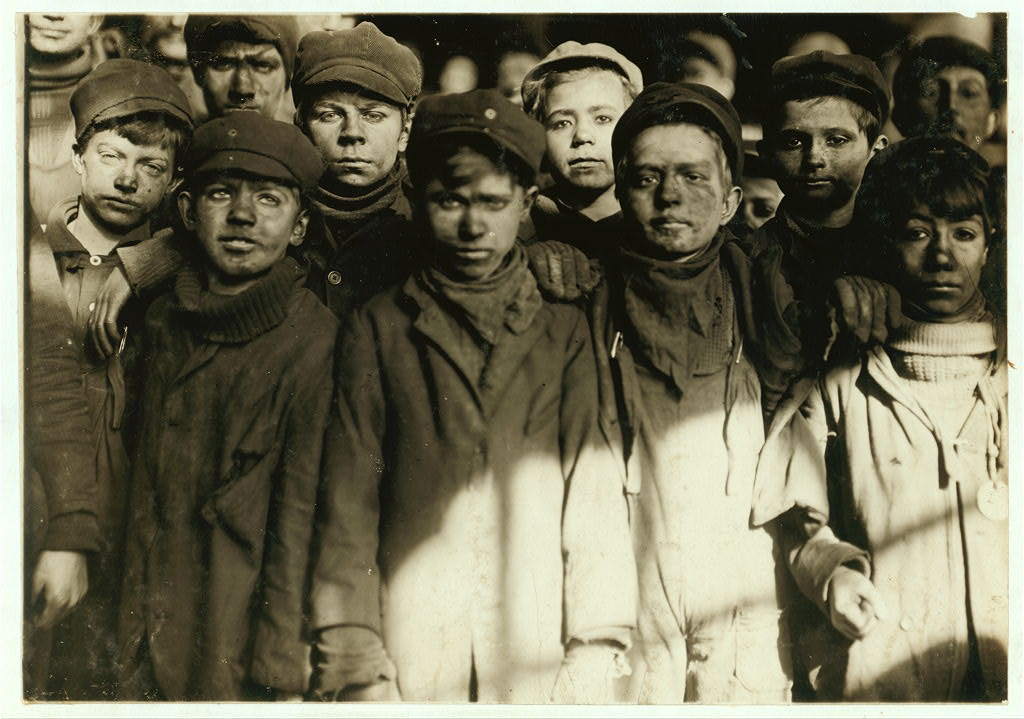
\includegraphics[width=0.62\linewidth]{images/book1/photos/g6-school-and-work-breaker-boys-1911.jpg}

{\small Boys who sorted coal at a mine in Pennsylvania, in the United States, in
1911. Photographs like this one were used in campaigns against \omterm{def:g6:school-and-work:child-labour}{child labour}.
(Photograph: Lewis Hine, 1911; Library of Congress; public domain.)}
\end{omfigure}

In the countries that took off first, children worked in fields, mines and
mills throughout the 1800s. The share of children at work fell as laws forbade
it, as schools became free and compulsory, and as families
became rich enough to do without their children's earnings.

% ledger: g6:ilo-child-labour-2000, g6:ilo-child-labour-2024, g6:ilo-child-labour-hazardous-2024,
% g6:ilo-child-labour-ssa-2024
\omterm{def:g6:school-and-work:child-labour}{Child labour} has not disappeared. The International Labour Organization and
UNICEF count it with household surveys. They estimate that about 246 million
children were in \omterm{def:g6:school-and-work:child-labour}{child labour} in 2000, and about 138 million in 2024 --- of
whom about 54 million in dangerous work, and about 87 million in Sub-Saharan
Africa, the region where families are poorest.

\section{Exercises}

\begin{exercise}[$\star$]\label{exo:g6:school-and-work:1}
Use the chart of literacy. About what share of the world's adults could read and
write in 1975, and in 2024?
\end{exercise}

\begin{exercise}[$\star$]\label{exo:g6:school-and-work:2}
Use the chart of hours worked. In 2023, in which of the six countries did
workers work the most hours? About how many?
\end{exercise}

\begin{exercise}[$\star$]\label{exo:g6:school-and-work:3}
A worker works 1\,800 hours in a year, spread over 45 working weeks (the other
weeks are holidays). How many hours does she work in a working week?
\end{exercise}

\begin{exercise}[$\star$]\label{exo:g6:school-and-work:4}
Use the chart of China's sectors. About what share of China's workers worked on
farms in 2000?
\end{exercise}

\begin{exercise}[$\star\star$]\label{exo:g6:school-and-work:5}
% figdata: hours_worked (deu 1950 2427, 2023 1335)
A German worker worked $2\,427$ hours in 1950 and $1\,335$ hours in 2023.
(a) Compute the \omterm{def:g6:reading-economic-charts:rate-of-change}{rate of change}, rounded to one decimal. (b) How many fewer hours
is that per week, over 52 weeks? Round to the nearest hour.
\end{exercise}

\begin{exercise}[$\star\star$]\label{exo:g6:school-and-work:6}
An invented country has 12 million workers; $35\,\%$ work in farming and
$25\,\%$ in industry. (a) How many work in each of the three sectors? (b) What
share works in services?
\end{exercise}

\begin{exercise}[$\star\star$]\label{exo:g6:school-and-work:7}
Use the chart of China's sectors. In about which year did the share of services
become larger than the share of farming? Explain how you see it on the chart.
\end{exercise}

\begin{exercise}[$\star\star$]\label{exo:g6:school-and-work:8}
Someone says: ``As a country gets richer, its people always work fewer hours.''
(a) Which line on the chart of hours worked contradicts this sentence for some
years? Which years? (b) Write a sentence about hours and income that the chart
does support.
\end{exercise}

\begin{exercise}[$\star\star$]\label{exo:g6:school-and-work:9}
In an invented country, 4.5 million women and 5.5 million men have paid work.
(a) What share of the workers are women? (b) Does this tell you what share of
women have paid work? What other number would you need?
\end{exercise}

\begin{exercise}[$\star\star\star$]\label{exo:g6:school-and-work:10}
% figdata: facts (women_lfp_1990 51.2, women_lfp_2025 48.9)
In the world, $51.2\,\%$ of women aged 15 and over were working or looking for
paid work in 1990, and $48.9\,\%$ in 2025. (a) By how many percentage points did
the share change? (b) Compute the \omterm{def:g6:reading-economic-charts:rate-of-change}{rate of change}, to one decimal. (c) Suggest
two explanations, and for each one the data that would check it.
\end{exercise}

\begin{exercise}[$\star\star\star$]\label{exo:g6:school-and-work:11}
An invented country had 600\,000 workers in 1990, $60\,\%$ of them on farms. In
2020 it has 900\,000 workers, $25\,\%$ of them on farms. (a) How many farm
workers were there at each date? (b) How many workers outside farming? (c) Did
the number of jobs outside farming grow faster or slower than the total number of
jobs?
\end{exercise}

\begin{exercise}[$\star\star\star$]\label{exo:g6:school-and-work:12}
The charts of this chapter show that people work fewer hours and fewer of them
work on farms. (a) Name two ways in which work could have become better that
these charts do not show. (b) Name one way in which it could have become worse.
(c) What data would you need to check one of them?
\end{exercise}

\section{Problem: Three Generations at Work}

\begin{problem}[{Weekend problem --- yearly hours of three generations, the
sectors they worked in, and what an hour of work bought them}]
\label{pb:g6:school-and-work:1}
A family of Brenland keeps its work diaries (everything is invented). The
grandfather, in 1965, worked 10 hours a day, 6 days a week, 50 weeks a year,
on a farm, for $0.50$ dalen an hour. The mother, in 1995, worked $8.5$ hours a day,
5 days a week, 47 weeks a year, in a factory, for 6 dalens an hour. The grandson,
in 2025, works 7 hours a day, 5 days a week, 46 weeks a year, in a hospital, for
20 dalens an hour. A simple bicycle cost 60 dalens in 1965, 180 dalens in 1995 and
300 dalens in 2025.

\medskip
\noindent\textbf{Part I --- Hours.}
\begin{enumerate}
  \item Compute each person's hours of work in a year.
  \item By how many percent did yearly hours fall from the grandfather to the
        grandson? Round to one decimal.
  \item The grandson's week is 35 hours. How many more hours a week did the
        grandfather work?
\end{enumerate}

\medskip
\noindent\textbf{Part II --- Sectors.} In Brenland, 50 workers in 100 worked on
farms in 1965, 30 in industry and 20 in services. In 2025, 8 work on farms, 22
in industry and 70 in services. Brenland had 400\,000 workers in 1965 and has
600\,000 in 2025.
\begin{enumerate}[resume]
  \item How many farm workers did Brenland have in 1965, and in 2025?
  \item How many service workers at each date?
  \item The number of farm workers fell. Does this mean that Brenland produces
        less food? What else would you need to know?
\end{enumerate}

\medskip
\noindent\textbf{Part III --- What an hour bought.}
\begin{enumerate}[resume]
  \item How many hours of work did a bicycle cost each person?
  \item How many bicycles could each person have bought with a full year's pay?
        Round to one decimal.
  \item From grandfather to grandson, yearly hours fell. Did the number of
        bicycles a year's work buys fall too? Explain.
  \item The mother's wage was 12 times the grandfather's. Was she 12 times
        better off? Use your answers to explain.
  \item Name two things about the three jobs that the diaries do not tell.
\end{enumerate}
\end{problem}
